%!TEX root = ../dokumentation.tex

\chapter{Introduction}\label{cha:Introduction}
??
\chapter{D1: Time estimate based on three point estimation}\label{cha:D1}
\begin{table}[H]
\centering
\caption{Three point estimation of effort for meeting requirements}
\begin{adjustbox}{width=1\textwidth, center=\textwidth}
\renewcommand{\arraystretch}{1}
\begin{tabular}{lllllll}
\textbf{Requirement} \textbf{Optimistic} & \textbf{Likely} & \textbf{Pessimistic} & \textbf{<T>} & \textbf{sigmahoch2} & \textbf{Actual}\\\hline
D1 & .& .& .& .& .&\\
\end{tabular}

\end{adjustbox}
\label{tbl:ConceptTPTPProductionSymbols}
\end{table}
\chapter{D2: Feasibility study}\label{cha:D2}
The aim of the feasibility study is to analyse whether the introduced model in section \ref{cha:Introduction} can be implemented based on the given formulas. 

\begin{equation}
	\frac{\partial v}{\partial t} = -c-b*p
\end{equation}
\begin{equation}
	\frac{\partial x}{\partial t} = v
\end{equation}

- Minimale Geschwindigkeit 0,29km/h beachten -> in m/s umrechnen \\
- Switch -> wenn Geschwindigkeit kleiner 0,29 folgt daraus Geschwindigkeit = 0 \\
- Screenshot Simulink Modell und Ergebnis\\
- R5 auch beachtet \\

\begin{figure}[H]
\centering
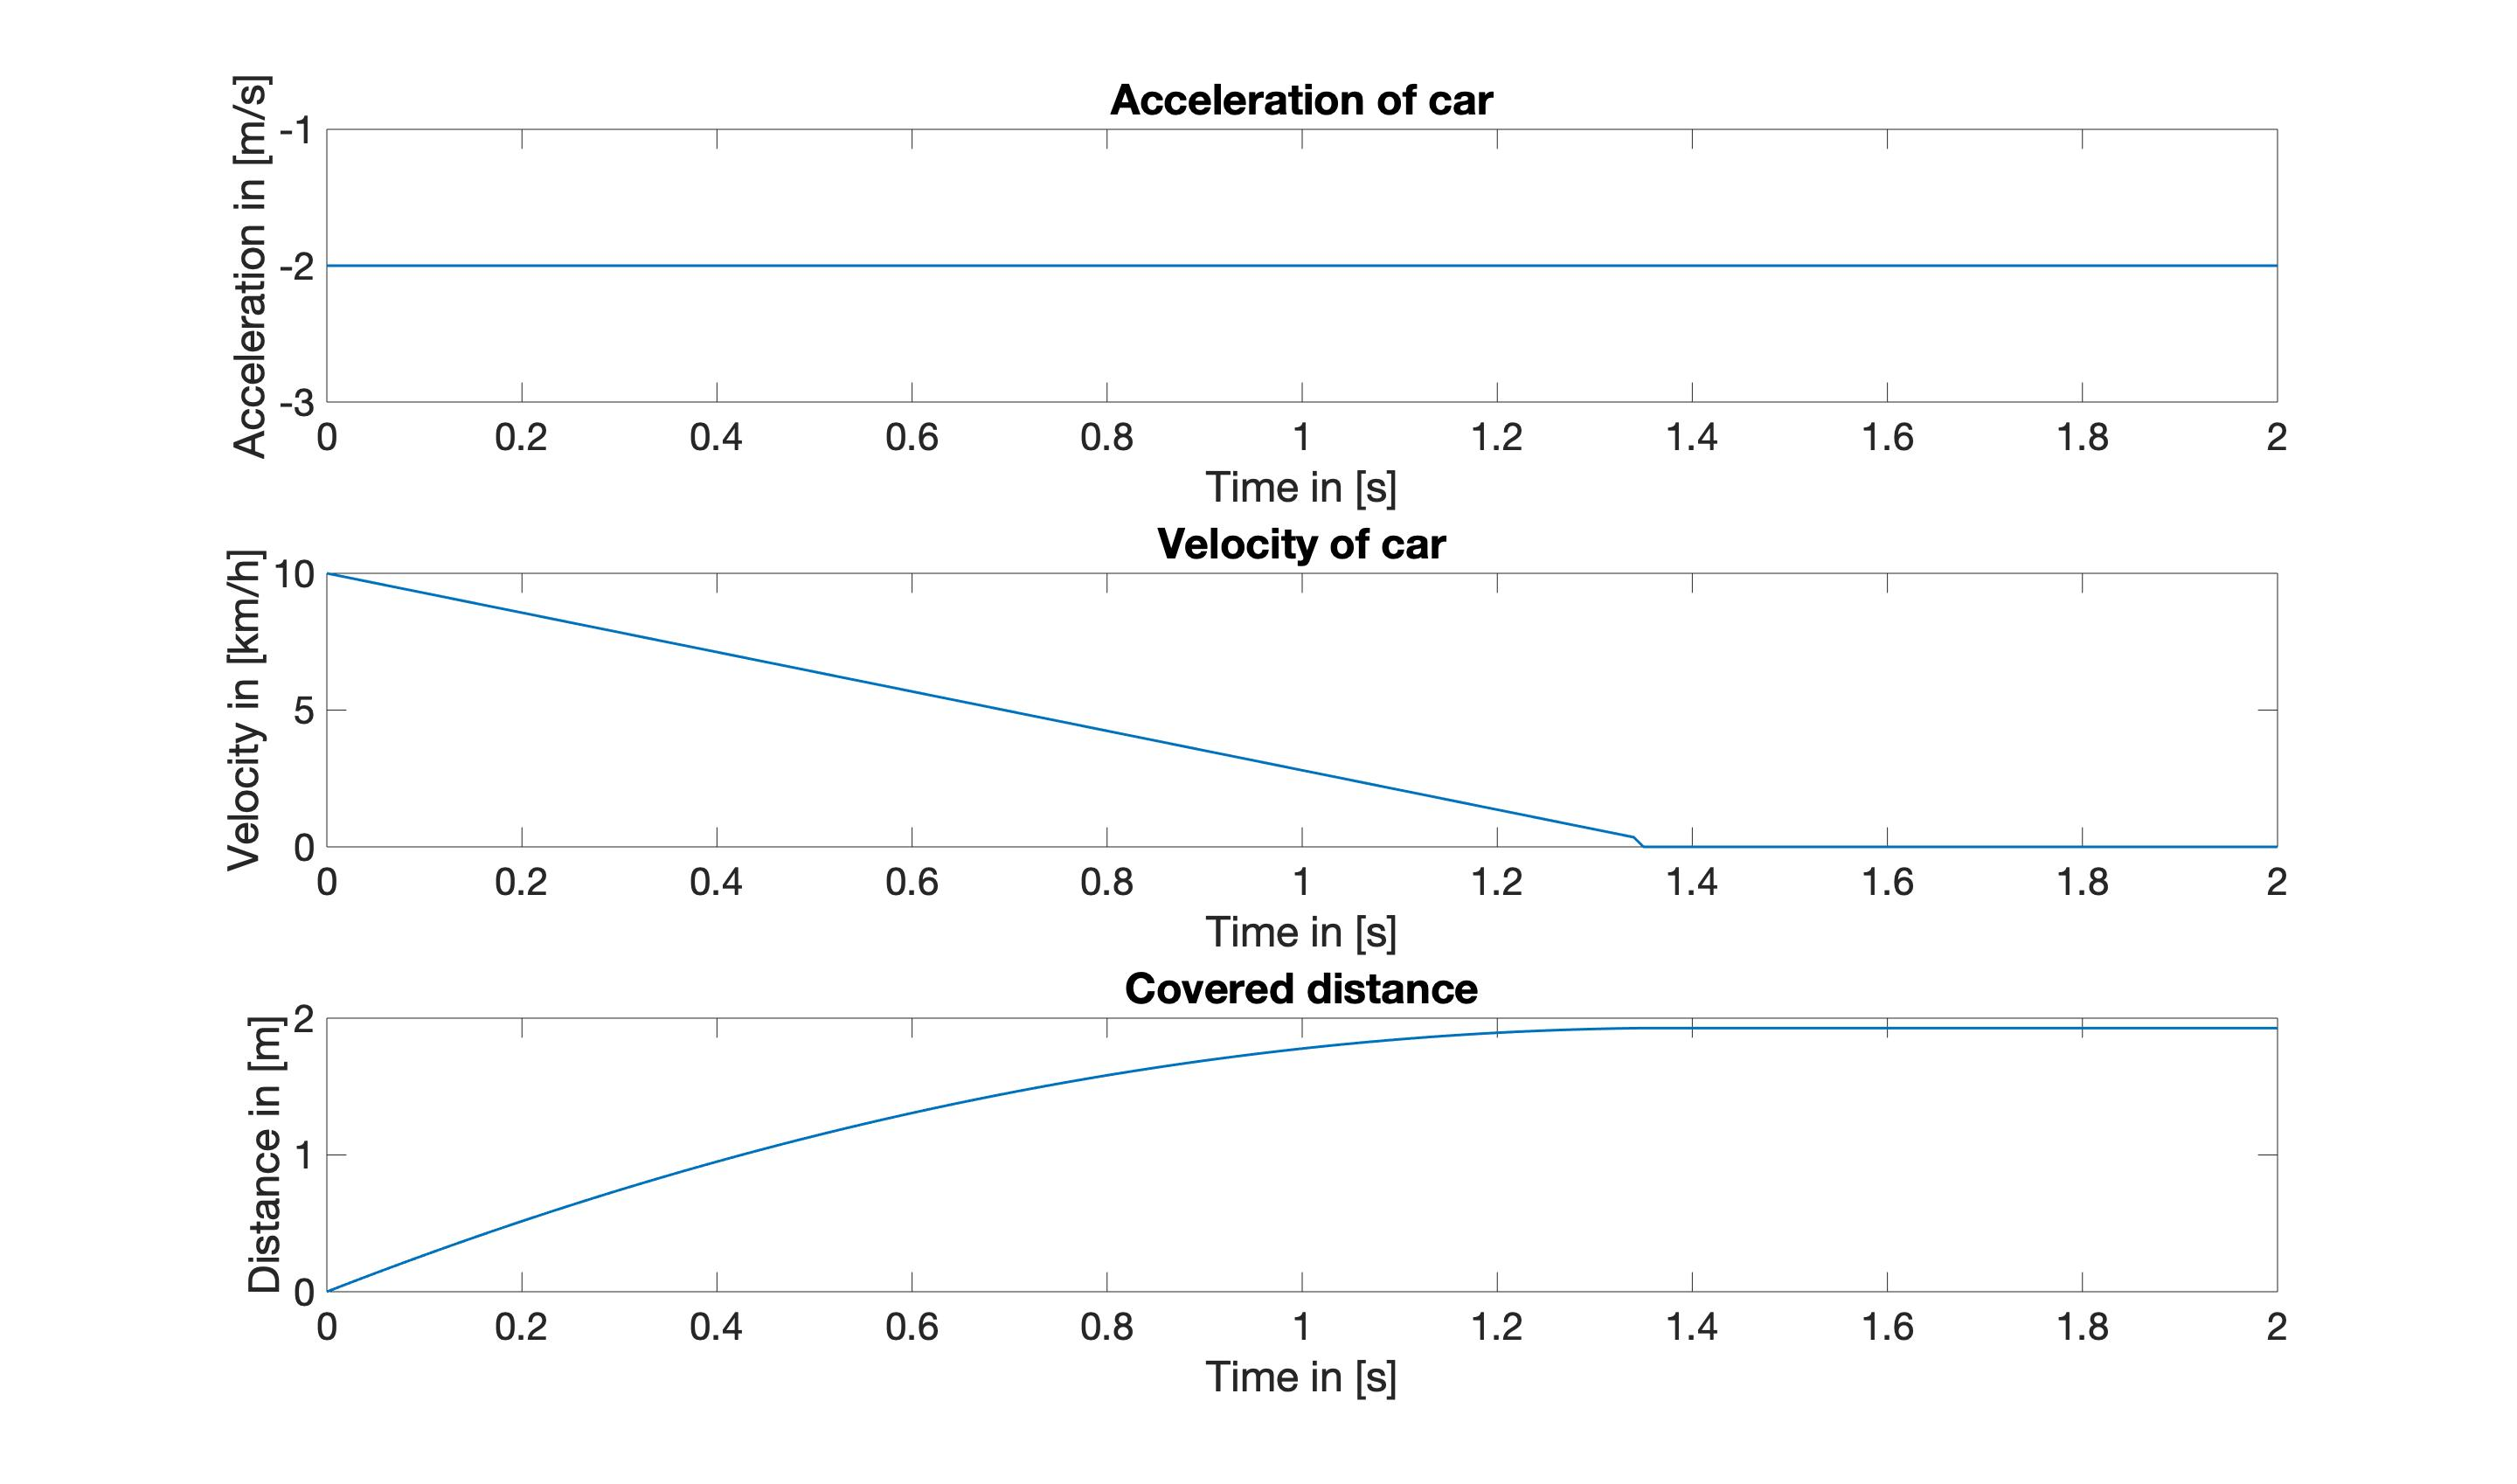
\includegraphics[width=1\textwidth]{images/D2_plot.jpg}
\caption{UML diagram of the architecture of the software tool}
\label{fig:ConceptArchitectureOverview}
\end{figure}

\begin{figure}[H]
\centering
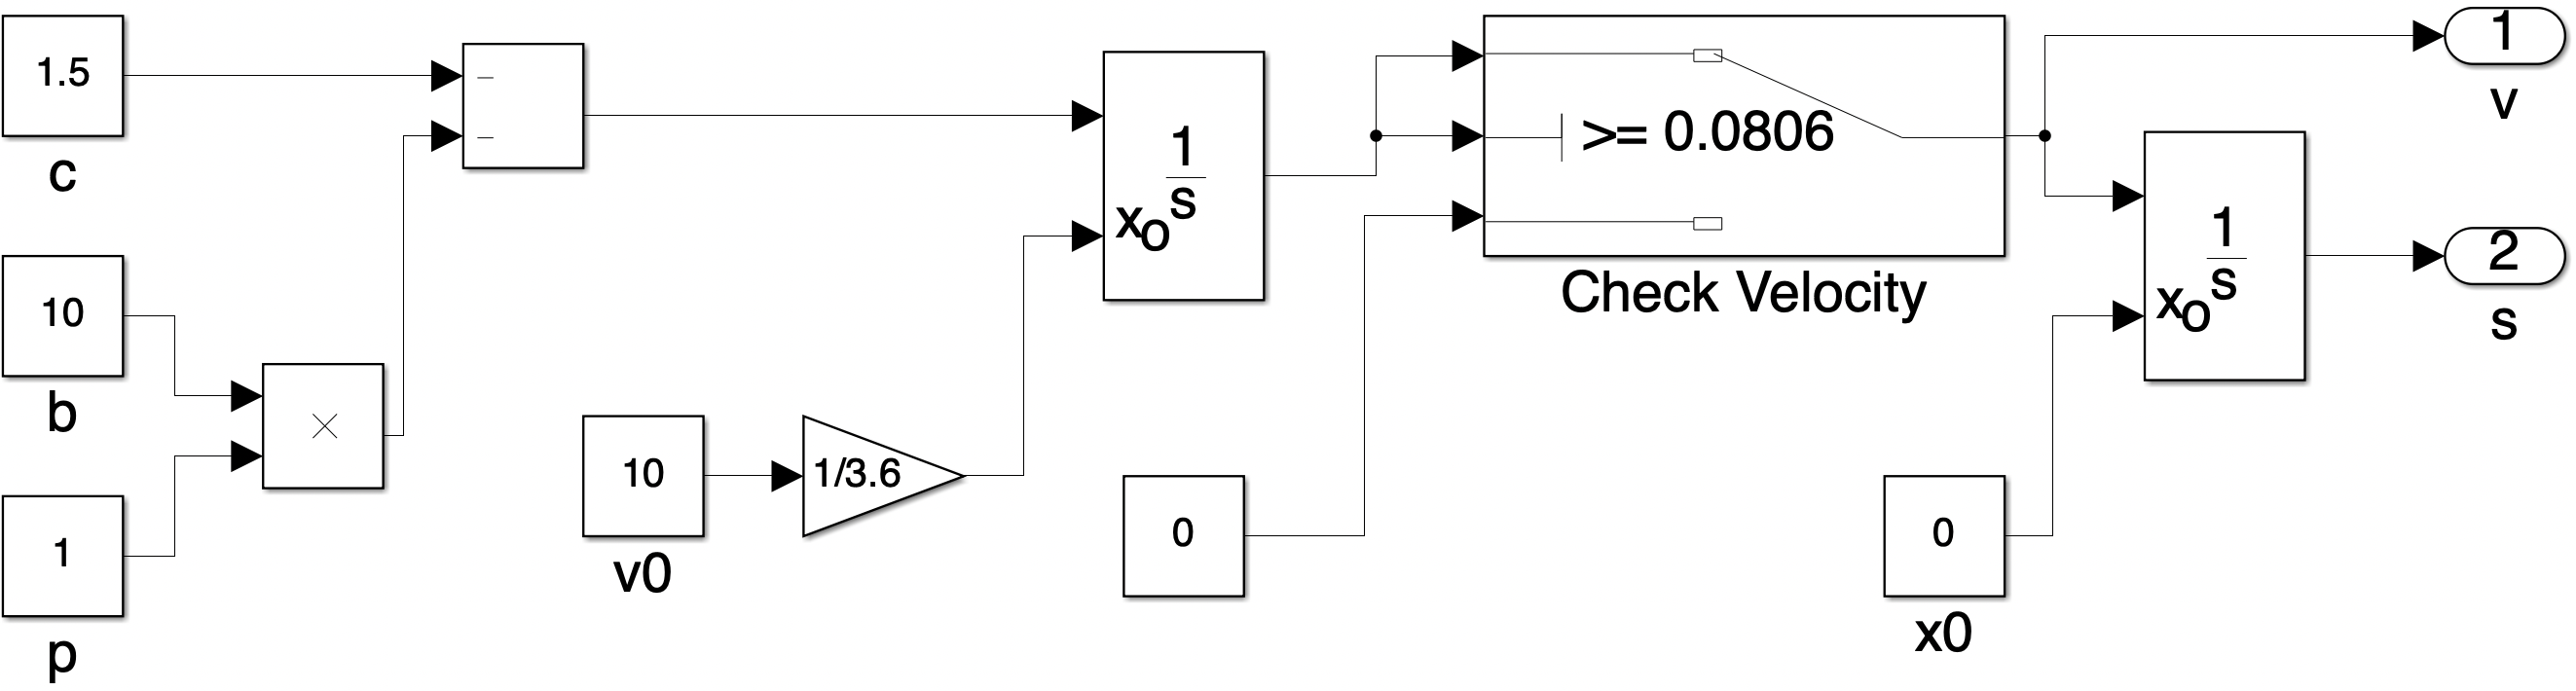
\includegraphics[width=1\textwidth]{images/D2_sim.png}
\caption{Simulink Modell der Differenzialgleichungen}
\label{fig:ConceptArchitectureOverview}
\end{figure}

\chapter{D3: Analysis of human velocity profile}\label{cha:D3}
1. Import in Matlab

2. entschieden Durchschnitt der vier Radgeschwindigkeiten zu nehmen (vllt. vor nachteile)
und so auf die Geschwindigkeit des Autos näherungsweise zu bestimmen

todo hier plot von gesamtgeschwindigkeit

idee: verzögerungsphasen extrahieren um so auf "menschliche" negative beschleunigung zu schließen
problem: verrauschte messdaten -> dadurch ständiger wehcsel positive negative beschleunigung

lösung: moving average filter zum glätten der messwerte
dann extrahieren der negativen beschleunigungen

\chapter{D4*: Consideration of uneven parking spaces}\label{cha:D4}

\chapter{D5: Discussion of inaccuracies in velocity measurement}\label{cha:D5}
validate findings by numbers from simulation

\chapter{D6: Implementation of pulse signal in Simulink}\label{cha:D6}

\chapter{D7: Transfer of Simulink model to ASCET}\label{cha:D7}

\chapter{D8: Implementation of pule signal in ASCET}\label{cha:D8}

\chapter{D9: Implementation of unit tests for ASCET model parts}\label{cha:D9}

\chapter{D10: Development and implementation of a system test environment for ASCET simulation}\label{cha:D10}

\chapter{D11*: Plausibility check comparing measured velocities and distances}\label{cha:D11}

\chapter{D13*: Impact of inaccuracies}\label{cha:D13}

\chapter{D14*: Reflection}\label{cha:D14}